\documentclass{standalone}

\usepackage{tikz}
\usepackage{standalone}

\begin{document}
    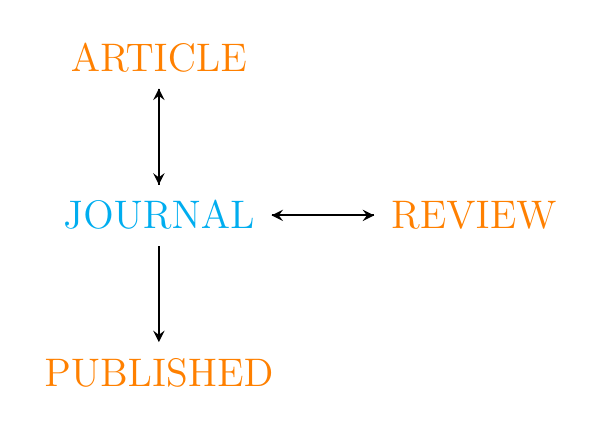
\begin{tikzpicture}

    \tikzstyle{state}=[minimum width=-0.2cm, font=\boldmath, inner sep=6pt];
	\tikzstyle{arrow} = [thick,->,>=stealth]

    \node[text=orange] (0) at (0, 0) [state]   {\Large{ARTICLE}};
    \node[text=cyan] (1) at (0, -2) [state]  {\Large{JOURNAL}};
    \node[text=orange] (2) at (4, -2) [state]  {\Large{REVIEW}};
    \node[text=orange] (3) at (0, -4) [state]  {\Large{PUBLISHED}};

	\draw [arrow] (0) -- (1);
	\draw [arrow] (1) -- (0);
	\draw [arrow] (1) -- (2);
	\draw [arrow] (2) -- (1);

	\draw [arrow] (1) -- (3);
	\end{tikzpicture}
\end{document}